\chapter{Re-examining the background-noise model}
\label{chap:reanalysis}

The failure analysis of \cref{chap:realdata} identified five distinct
causes of distribution shift between the synthetic training set and
the real 2015 recordings. Before re-implementing the data generator,
we return to the four months of real data and ask the question that
the original calibration of \cref{sec:stat-charac} did not pose: how
good a description of the background signal is the noise model
\cref{eq:noise-model} that the current generator relies on?

This chapter is deliberately narrow in scope: we restrict attention to
the \emph{background} component of the signal --- the process that the
network sees $\sim 99\%$ of the time at deployment --- and ask whether
the assumed model (IID Gaussian fluctuations on an Ornstein--Uhlenbeck
baseline) actually matches it. The answer is negative on two distinct
points: the high-frequency fluctuation is autocorrelated rather than
white (\cref{sec:reanal-noise,sec:reanal-arorder}), and the baseline
shows systematic linear trends rather than mean-reverting random
walks (\cref{sec:reanal-drift}). Both turn into concrete changes for
the next iteration of the generator (\cref{sec:reanal-targets}).

The analysis is in
\texttt{data-gen/analyze\_noise\_model.py}: outlier-masking, AR order
selection, whitening tests, innovation distribution, parameter
stability, and the linear-drift fit on the ultra-wide baseline.
Numerical artifacts land under
\texttt{data-gen/logs/noise\_analysis/}.

\section{Methodology}
\label{sec:reanal-method}

The original calibration estimated the high-frequency noise standard
deviation as the sample standard deviation of the moving-average
residual, over the entire month. Two methodological refinements are
needed before the inferred statistics can be trusted:

\paragraph{Robust outlier masking.}
The signal contains visible excursions whose amplitudes inflate the
sample standard deviation and distort the empirical autocorrelation.
We use a rolling Median Absolute Deviation (MAD) for the local
dispersion estimate (breakdown point $50\%$) and mask samples whose
robust z-score exceeds $4$ before computing residual statistics. The
robust z-score is
\begin{equation}
    z_t = \frac{x_t - b_t}{1.4826 \cdot \mathrm{MAD}_w(x - b)_t},
    \label{eq:robust-z}
\end{equation}
with $b_t$ the centred moving-average baseline and $1.4826 =
1/\Phi^{-1}(0.75)$ the standard scaling factor that makes the
MAD a consistent estimator of the standard deviation under Gaussian
assumptions. We make no claim about the physical nature of the
flagged samples; the goal of the masking is solely to isolate a
\emph{clean} fraction of the signal on which to fit the noise model.

\paragraph{Multi-scale baseline.}
The single $w = 480$ moving average used in \cref{sec:stat-charac}
absorbs features whose duration is comparable to or shorter than $w$.
We use $w_s = 480$ for the high-frequency residual analysis and an
ultra-wide $w_w = 17\,280$ baseline (\emph{i.e.}\ $\sim 12$ days) for
the drift analysis of \cref{sec:reanal-drift}.

After masking, $\sim 95$--$99\%$ of each month survives as the
\emph{clean residual}, on which all noise statistics below are
computed.

\section{High-frequency noise: AR(1) is good, white is wrong}
\label{sec:reanal-noise}

\Cref{fig:reanal-clean-residual} shows the diagnostic plot computed on
the masked residual of February 2015. The histogram and the Q-Q plot
are both essentially perfect Gaussian fits --- the marginal
distribution of the clean residual is, to a very good approximation,
$\mathcal{N}(0, \sigma^2)$. That part of \cref{eq:noise-model} is
correct.

\begin{figure}[H]
    \centering
    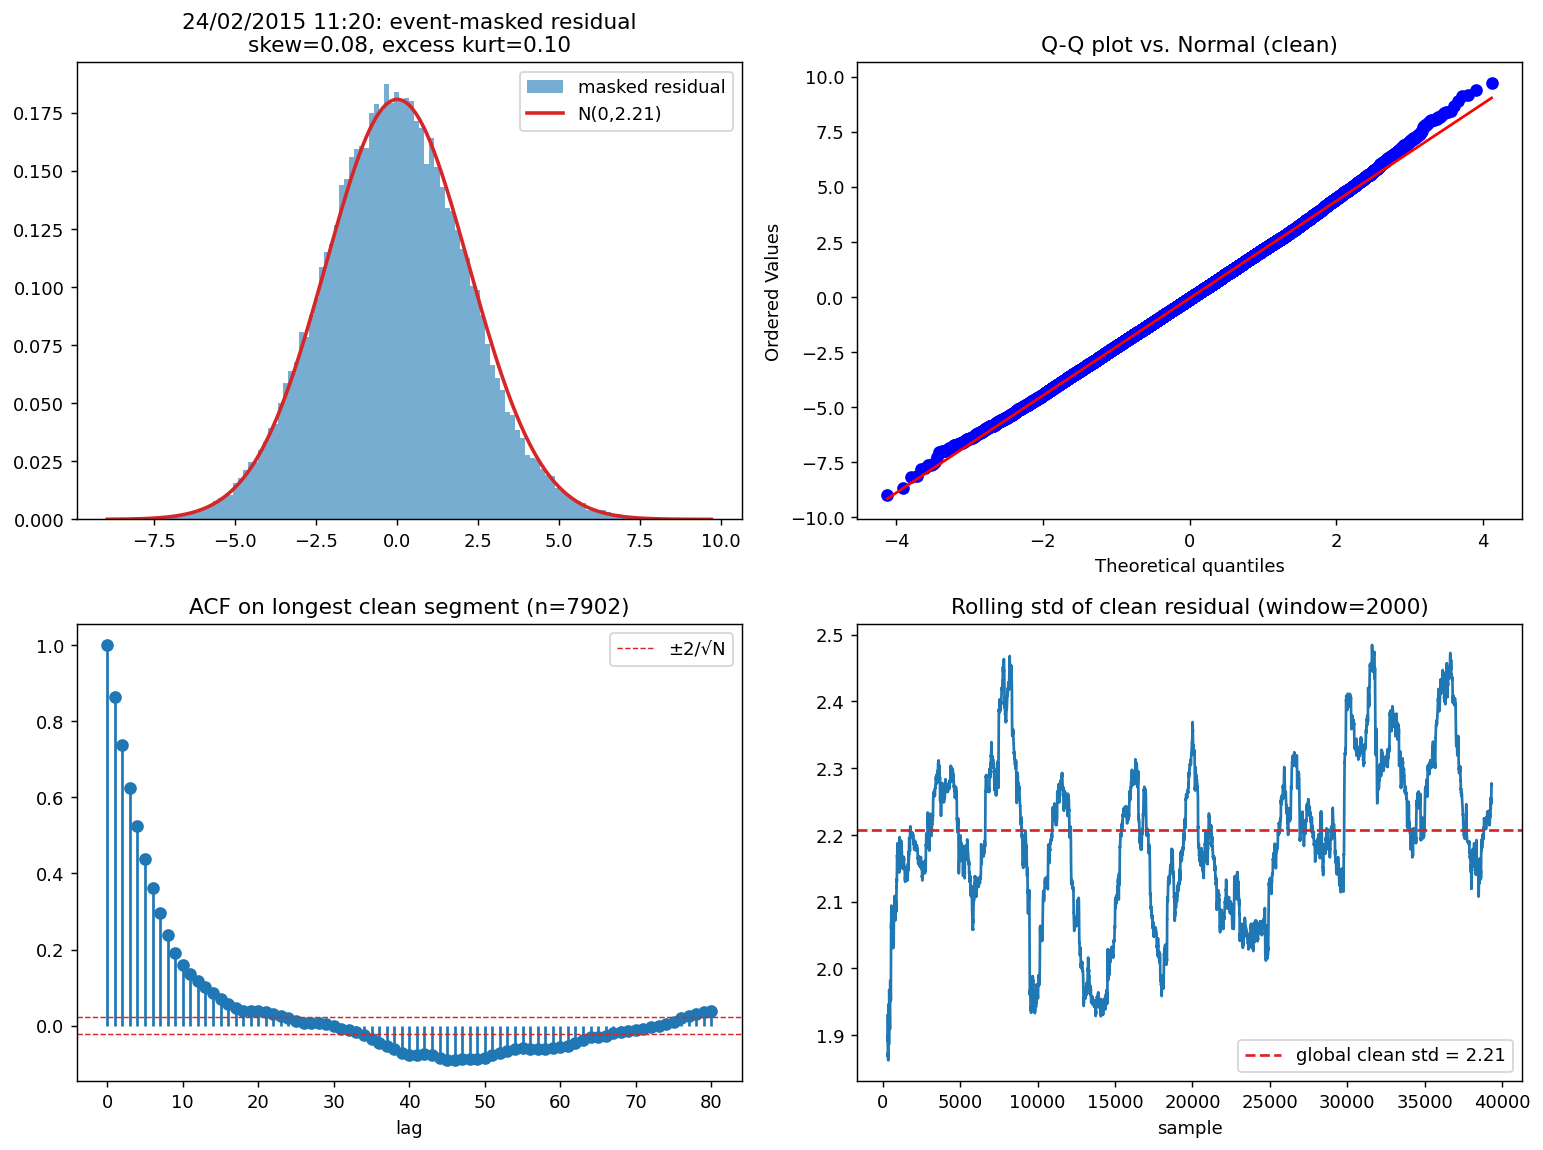
\includegraphics[width=\linewidth]{figures/real_reanalysis_clean_residual}
    \caption{Diagnostics on the masked residual of February 2015
    (clean fraction $93\%$). Top-left: histogram, near-perfectly fit
    by $\mathcal{N}(0, 2.21)$ (red). Top-right: Q-Q plot vs.\ Normal,
    on the diagonal. Bottom-left: autocorrelation function on the
    longest contiguous clean segment --- $\mathrm{ACF}(1) = 0.864$,
    decaying smoothly to zero by lag $\sim 30$. Bottom-right:
    rolling-window standard deviation, stationary around the global
    value. The marginal distribution agrees with the IID-Gaussian
    assumption of \cref{eq:noise-model}; the autocorrelation does
    not.}
    \label{fig:reanal-clean-residual}
\end{figure}

The autocorrelation panel, however, is not. Under an IID-Gaussian
residual, $\mathrm{ACF}(k)$ should sit inside the $\pm 2/\sqrt{N}$ band
for all $k \geq 1$. The empirical ACF instead starts at $0.864$ at
lag $1$ and decays smoothly to zero only around lag $30$.
\Cref{tab:reanal-noise} confirms that the same pattern holds in every
month.

\begin{table}[H]
    \centering
    \footnotesize
    \begin{tabular}{lcccccc}
        \toprule
        Month & Clean frac.\ & $\sigma$ & Skew & Exc.\ kurt &
        $\mathrm{ACF}(1)$ & AR(1) $\varphi$ \\
        \midrule
        24/02/2015 & $0.927$ & $2.21$ & $+0.08$ & $+0.10$ & $0.864$ & $0.864$ \\
        30/04/2015 & $0.909$ & $2.34$ & $+0.22$ & $+1.01$ & $0.867$ & $0.867$ \\
        22/06/2015 & $0.953$ & $2.36$ & $+0.60$ & $+3.74$ & $0.850$ & $0.850$ \\
        20/10/2015 & $0.917$ & $2.30$ & $+0.24$ & $+1.07$ & $0.861$ & $0.861$ \\
        \midrule
        \textbf{Average} & $0.927$ & $2.30$ & $+0.29$ & $+1.48$ &
        $\mathbf{0.861}$ & $\mathbf{0.861}$ \\
        \bottomrule
    \end{tabular}
    \caption{Event-masked residual statistics. ACF$(1)$ and the
    fitted AR(1) coefficient are numerically identical: the
    maximum-likelihood estimator of $\varphi$ in a Gaussian AR(1)
    \emph{is} the lag-1 autocorrelation. The marginal standard
    deviation $\sigma = 2.30$ matches the value reported in
    \cref{tab:real-stats}; what \cref{tab:real-stats} did not see
    is the strong serial correlation behind it.}
    \label{tab:reanal-noise}
\end{table}

The clean residual is well described by a first-order autoregressive
Gaussian process,
\begin{equation}
    r_t = \varphi\, r_{t-1} + \varepsilon_t,
    \quad \varepsilon_t \overset{\text{iid}}{\sim} \mathcal{N}(0, \sigma_\varepsilon^2),
    \quad \varphi \approx 0.86,
    \label{eq:ar1-noise}
\end{equation}
with stationary marginal variance
$\sigma_r^2 = \sigma_\varepsilon^2 / (1 - \varphi^2)$. Plugging
$\sigma_r = 2.30$ and $\varphi = 0.86$ gives an innovation standard
deviation $\sigma_\varepsilon \approx 1.17$, and an effective
correlation length $\tau \approx 1 / (1 - \varphi) \approx 7$ samples.

\paragraph{Why this matters.}
The current generator uses $\varphi = 0$, \emph{i.e.}\ white noise. A
sliding window of size $W = 512$ samples therefore sees a
fundamentally different noise texture in synthetic vs.\ real data:
the synthetic window looks ``rougher'' (independent samples), while
the real window is substantially smoother on short scales because of
the autoregressive memory. The marginal histogram of values inside
the window is identical in the two cases (both Gaussian with
$\sigma \approx 2.3$), so any model that looks only at the marginal
distribution sees no shift; but a 1D convolutional layer, which
extracts features from local patches of a few samples, sees a
fundamentally different input. This is an additional component of
the distribution shift that the original failure analysis did not
isolate.

\section{Is AR(1) enough? AR-order selection and whitening}
\label{sec:reanal-arorder}

Equation \cref{eq:ar1-noise} is the simplest model consistent with the
short-lag autocorrelation, but a higher-order autoregressive process
could in principle fit the data better. We test this by fitting
AR(p) on the clean residual for $p \in \{1, 2, 3, 5, 10\}$ and
comparing AIC, BIC, and the whiteness of the residual innovations.

\subsection{AR-order selection}

\Cref{tab:reanal-ar-order} reports the AIC and BIC for each fitted
order, averaged across the four months. The differences between
orders are small (the absolute values of AIC/BIC differ by less than
$0.05\%$ between $p = 1$ and $p = 10$), but consistent enough across
months for the pattern to be unambiguous: BIC, which penalises
higher orders more heavily, selects $\mathrm{AR}(1)$ in three months
out of four and $\mathrm{AR}(2)$ in October. AIC, which is more
lenient, prefers $\mathrm{AR}(10)$ everywhere --- but with
$N \approx 38\,000$ samples per month, AIC over-fits readily.

\begin{table}[H]
    \centering
    \footnotesize
    \begin{tabular}{ccccc}
        \toprule
        $p$ & $\varphi_1$ & $\varphi_2$ & $\varphi_3$ & $\sigma_\varepsilon$ \\
        \midrule
        $1$  & $+0.864$ & ---      & ---      & $1.119$ \\
        $2$  & $+0.878$ & $-0.015$ & ---      & $1.119$ \\
        $3$  & $+0.879$ & $-0.022$ & $+0.007$ & $1.119$ \\
        $5$  & $+0.879$ & $-0.022$ & $+0.006$ & $1.119$ \\
        $10$ & $+0.879$ & $-0.022$ & $+0.006$ & $1.119$ \\
        \bottomrule
    \end{tabular}
    \caption{First few AR coefficients of AR(p) fits to the clean
    residual, averaged across the four months. Higher-order
    coefficients are essentially zero. The innovation standard
    deviation is invariant across orders. AR(2) captures the only
    appreciable correction to AR(1): a small negative
    $\varphi_2 \approx -0.02$, consistent with a mild ``overshoot''
    after a positive sample.}
    \label{tab:reanal-ar-order}
\end{table}

\subsection{Whitening: are AR innovations white?}
\label{sec:reanal-whitening}

A more direct test of model adequacy is whether the AR innovations
themselves are white noise. We use the Ljung--Box portmanteau test:
$Q = N(N + 2) \sum_{k=1}^{K} \hat{\rho}_k^2 / (N - k)$ is
$\chi^2_{K - p}$-distributed under the null that the innovations have
no residual autocorrelation. The results are summarised in
\cref{tab:reanal-ljungbox}.

\begin{table}[H]
    \centering
    \footnotesize
    \begin{tabular}{lcccccc}
        \toprule
        & \multicolumn{2}{c}{February} & \multicolumn{2}{c}{June} &
        \multicolumn{2}{c}{October} \\
        \cmidrule(lr){2-3}\cmidrule(lr){4-5}\cmidrule(lr){6-7}
        Order $p$ & LB(20) & LB(50) & LB(20) & LB(50) & LB(20) & LB(50) \\
        \midrule
        $1$  & $0.010$ & $0.13$ & $0.046$ & $0.018$ & $0.018$ & $0.16$ \\
        $2$  & $0.040$ & $0.26$ & $0.144$ & $0.049$ & $0.16$  & $0.43$ \\
        $3$  & $0.041$ & $0.26$ & $0.21$  & $0.07$  & $0.27$  & $0.56$ \\
        $5$  & $0.045$ & $0.28$ & $0.53$  & $0.16$  & $0.56$  & $0.75$ \\
        $10$ & $0.93$  & $0.95$ & $0.99$  & $0.51$  & $0.95$  & $0.95$ \\
        \bottomrule
    \end{tabular}
    \caption{Ljung--Box $p$-values on AR(p) innovations at $20$ and
    $50$ lags. The null hypothesis (innovations are white) is rejected
    at the $5\%$ level when the $p$-value is below $0.05$. April is
    omitted because its much shorter clean segment gives high
    p-values for every order (the test has low power). With $N
    \approx 38\,000$ samples per month, even very small residual
    autocorrelations are detectable, which is why AR(1) is formally
    rejected in three months out of four. AR(2) is borderline; AR(5)
    accepts whiteness everywhere except at LB(50) for June. AR(10)
    is clearly white.}
    \label{tab:reanal-ljungbox}
\end{table}

The pattern is consistent: AR(1) is formally rejected by Ljung--Box,
AR(2)--AR(5) are borderline, AR(10) is clearly white. \emph{However},
the AR coefficients beyond $\varphi_2$ are essentially zero
(\cref{tab:reanal-ar-order}); the improvement from higher orders is
the typical large-$N$ artifact where statistically detectable but
practically negligible residual structure crosses the rejection
threshold. The visual ACF of \cref{fig:reanal-ar1-innov}, bottom-left,
makes this concrete: the AR(1) innovations have ACF bars
indistinguishable from zero at every visible lag.

\begin{figure}[H]
    \centering
    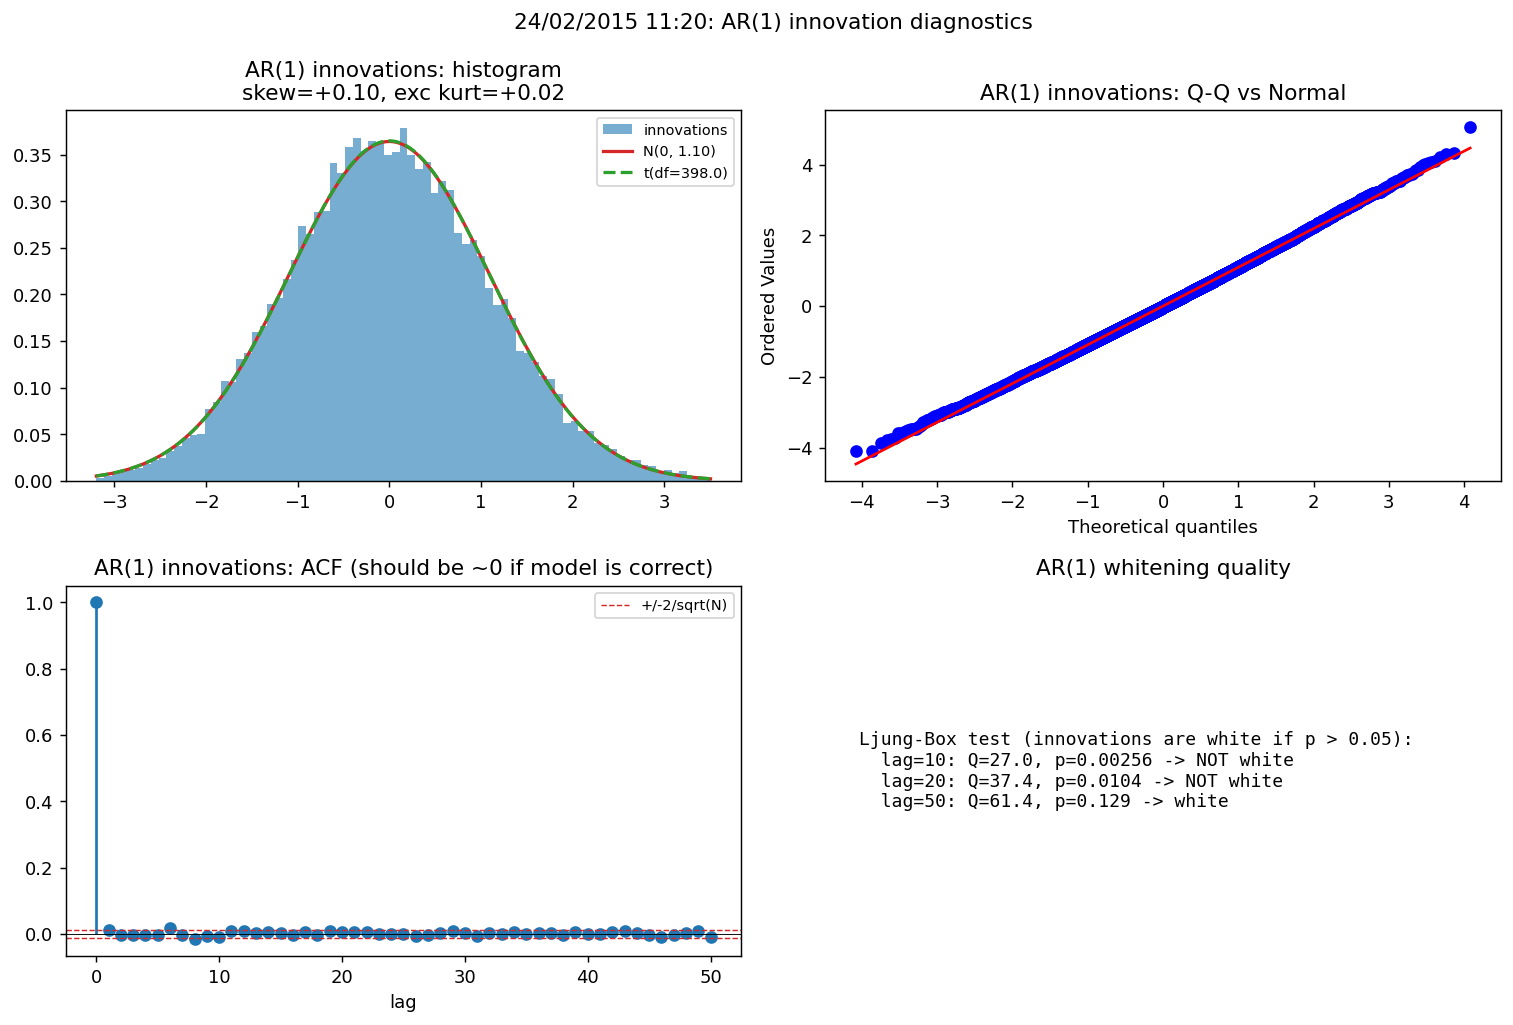
\includegraphics[width=\linewidth]{figures/real_reanalysis_ar1_innov}
    \caption{AR(1) innovation diagnostics for February 2015.
    Top-left: histogram of the innovations, with $\mathcal{N}(0,
    1.10)$ (red) and a fitted Student-$t$ (green dashed,
    $\nu = 398$, so essentially Gaussian). Top-right: Q-Q plot vs.\
    Normal, on the diagonal. Bottom-left: ACF of the innovations ---
    all bars within or barely outside the $\pm 2/\sqrt{N}$ band.
    Bottom-right: Ljung--Box test summary; the formal rejection of
    whiteness at LB(10) is driven by a residual ACF of $\sim 0.02$,
    which is statistically detectable at $N = 38\,000$ but
    practically irrelevant.}
    \label{fig:reanal-ar1-innov}
\end{figure}

\Cref{fig:reanal-psd-cmp} confirms the same conclusion from a
frequency-domain angle: the empirical periodogram is matched almost
identically by the theoretical PSD of every AR order considered.

\begin{figure}[H]
    \centering
    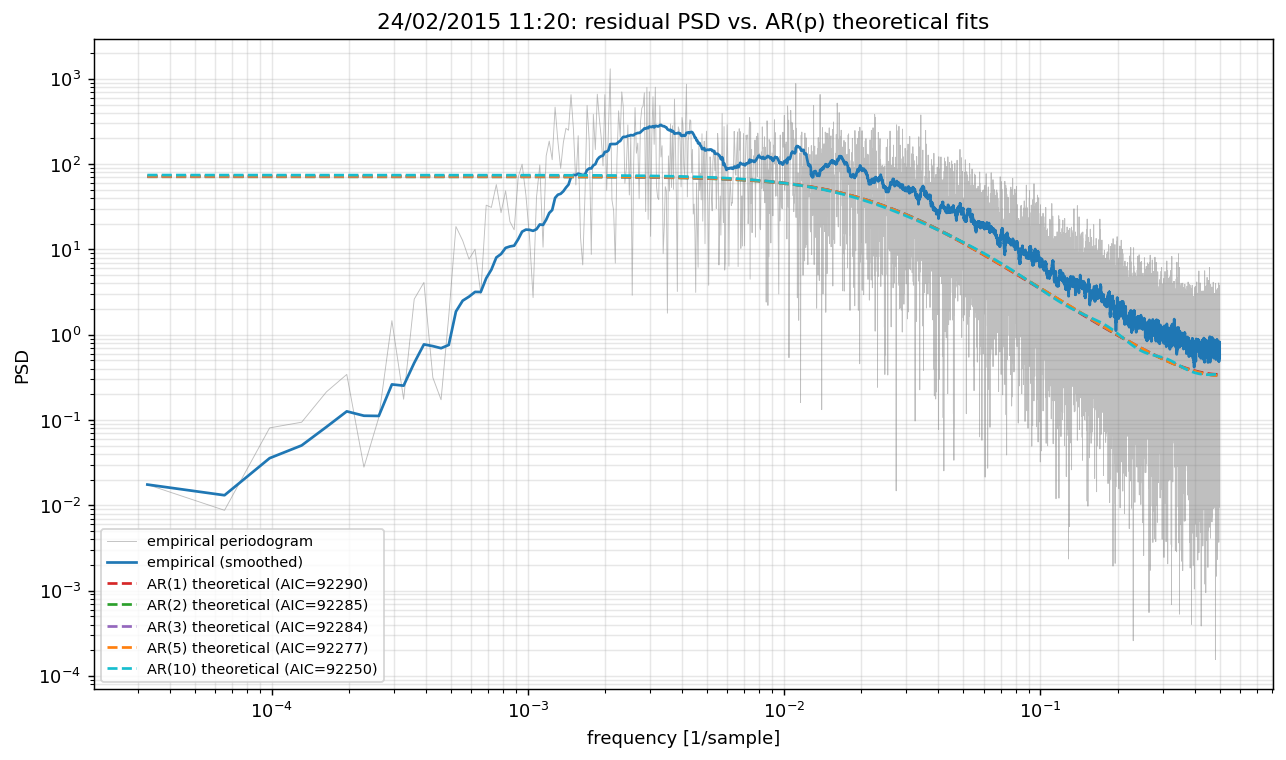
\includegraphics[width=0.85\linewidth]{figures/real_reanalysis_psd_cmp}
    \caption{Empirical residual PSD of February 2015 (grey scatter +
    blue smoothed line) against the theoretical PSDs of the fitted
    AR(p) models (dashed coloured lines). AR(1), AR(2), AR(3), AR(5)
    and AR(10) produce essentially indistinguishable theoretical
    spectra, all of which match the empirical periodogram across
    five orders of magnitude in frequency.}
    \label{fig:reanal-psd-cmp}
\end{figure}

\subsection{Innovation distribution}

The AR(1) innovations are very accurately Gaussian. The skew is
$+0.06$--$+0.10$ and the excess kurtosis is $-0.06$--$+0.10$ across
the four months. A maximum-likelihood fit of a Student-$t$ returns
$\nu \in [69, 6900]$ depending on the month, i.e.\ effectively
infinity (Student-$t$ converges to Normal as $\nu \to \infty$). The
generator can therefore use Gaussian innovations without any
qualification.

\subsection{Stationarity of \texorpdfstring{$\varphi$}{phi} and
\texorpdfstring{$\sigma_\varepsilon$}{sigma\_eps}}

Splitting each month into four equal-length chunks and re-fitting
AR(1) on each gives the values reported in
\cref{tab:reanal-stability} and visualised in
\cref{fig:reanal-stability}. The estimates are stable to within
$\pm 0.04$ for $\varphi$ and $\pm 0.05$ for $\sigma_\varepsilon$. The
first chunk has a slightly elevated $\varphi$, consistent with a
small fraction of residual unmasked outliers in the early part of
each recording.

\begin{table}[H]
    \centering
    \footnotesize
    \begin{tabular}{lcccc}
        \toprule
        Month & $\varphi$ Q1 & $\varphi$ Q2 & $\varphi$ Q3 & $\varphi$ Q4 \\
        \midrule
        24/02/2015 & $0.891$ & $0.875$ & $0.864$ & $0.878$ \\
        30/04/2015 & $0.945$ & $0.865$ & $0.866$ & $0.866$ \\
        22/06/2015 & $0.877$ & $0.859$ & $0.851$ & $0.909$ \\
        20/10/2015 & $0.924$ & $0.847$ & $0.861$ & $0.867$ \\
        \bottomrule
    \end{tabular}
    \caption{AR(1) coefficient $\varphi$ refitted on each quarter of
    each month. The estimates are tightly clustered around the
    aggregate value $\varphi \approx 0.86$, with the largest excursion
    in Q1 of April ($\varphi = 0.945$, almost certainly contaminated
    by the cluster of unmasked excursions at the start of that
    recording). The generator can safely use a single
    $\varphi \approx 0.86$ without sampling it per recording.}
    \label{tab:reanal-stability}
\end{table}

\begin{figure}[H]
    \centering
    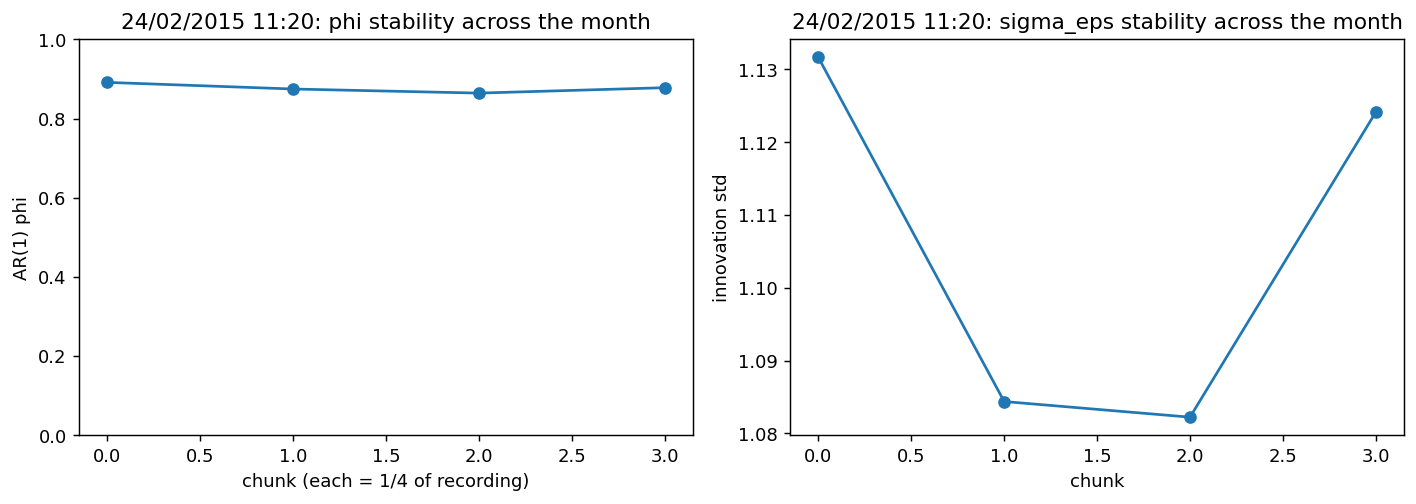
\includegraphics[width=0.85\linewidth]{figures/real_reanalysis_stability}
    \caption{Per-quarter AR(1) parameter estimates for February 2015.
    The left panel shows $\varphi$ (essentially constant at
    $\sim 0.87$); the right panel shows the innovation standard
    deviation $\sigma_\varepsilon$ (constant at $\sim 1.10$).}
    \label{fig:reanal-stability}
\end{figure}

\subsection{Take-away}

The high-frequency noise is well modelled by a stationary
$\mathrm{AR}(1)$ Gaussian process with
\begin{equation}
    \varphi = 0.86, \qquad \sigma_\varepsilon = 1.12, \qquad
    \sigma_r = \sigma_\varepsilon / \sqrt{1 - \varphi^2} = 2.30.
    \label{eq:final-noise-params}
\end{equation}
An AR(2) refinement with $\varphi_2 \approx -0.02$ marginally improves
the fit but is, for all practical purposes, indistinguishable from
AR(1) at the texture scale that the convolutional network sees. The
generator should therefore replace the current $\varphi = 0$ assumption
by \cref{eq:final-noise-params}.

\section{Baseline drift: linear, not mean-reverting}
\label{sec:reanal-drift}

The Ornstein--Uhlenbeck baseline of \cref{eq:noise-model} is a
\emph{stationary} mean-reverting random walk: its long-run mean is
$\mu$ and its variance is bounded by
$\sigma_{\mathrm{OU}}^2 / (2\theta)$. With the parameters in
\cref{tab:real-stats}, this gives an equilibrium standard deviation
of $\sim 13$ --- large enough that the OU process can in principle
wander, but only as a stationary random walk, not as a systematic
drift.

\Cref{tab:reanal-drift} reports a linear fit to the wide-scale
baseline of each month (a moving average over $w = 17{,}280$ samples,
\emph{i.e.}\ $\sim 12$ days, which absorbs anything but the seasonal
trend).

\begin{table}[H]
    \centering
    \footnotesize
    \begin{tabular}{lccc}
        \toprule
        Month & Linear slope / sample & Total drift over $\sim 40\text{k}$ samples
              & ADF $p$-value \\
        \midrule
        24/02/2015 & $+7.5 \cdot 10^{-5}$ & $+2.95$ & $0.159$ \\
        30/04/2015 & $+2.1 \cdot 10^{-5}$ & $+0.84$ & $1.9 \cdot 10^{-9}$ \\
        22/06/2015 & $+9.8 \cdot 10^{-5}$ & $+3.87$ & $0.104$ \\
        20/10/2015 & $-1.0 \cdot 10^{-4}$ & $-3.99$ & $1.6 \cdot 10^{-3}$ \\
        \bottomrule
    \end{tabular}
    \caption{Wide-scale baseline drift per month. The fourth column is
    the augmented Dickey--Fuller test $p$-value (the null is a unit
    root, \emph{i.e.}\ non-stationary). The OU model would correspond
    to a \emph{stationary} baseline; ADF rejects stationarity in two
    months out of four, and the systematic linear slopes
    ($\pm 3$ counts per month) cannot be reproduced by the OU process
    with the fitted $(\theta, \sigma_{\mathrm{OU}})$.}
    \label{tab:reanal-drift}
\end{table}

The slopes are of order $10^{-4}$ counts per sample and their sign
varies across months, consistent with seasonal or meteorological
trends rather than mean-reverting noise. An OU process simulating a
month-long path is overwhelmingly likely to return close to its
starting point; the real baseline does not.

\section{Updated background model and acceptance test}
\label{sec:reanal-targets}

Putting \cref{sec:reanal-noise,sec:reanal-arorder,sec:reanal-drift}
together, the background signal in the next iteration of the generator
should be
\begin{equation}
    x_t = a + s \cdot t + b_t + r_t,
    \label{eq:reanal-bg-model}
\end{equation}
where
\begin{itemize}[leftmargin=*, itemsep=0.2em]
    \item $a$ is a per-recording offset, sampled around the empirical
    global mean $\mu \approx 99.3$;
    \item $s$ is a per-recording linear slope, sampled from
    $\mathcal{N}(0, \sigma_s^2)$ with $\sigma_s \approx 10^{-4}$
    counts per sample, so the typical total drift over a recording
    matches the $\pm 3$--$4$ counts of \cref{tab:reanal-drift};
    \item $b_t$ is the OU residual baseline of \cref{eq:noise-model}
    with $\theta = 4 \cdot 10^{-6}$ and a re-fitted
    $\sigma_{\mathrm{OU}}$ tuned so that the combined drift
    $s \cdot t + b_t$ matches the empirical wide-scale baseline range
    of \cref{tab:reanal-drift};
    \item $r_t$ is the AR(1) Gaussian noise of
    \cref{eq:ar1-noise,eq:final-noise-params} with
    $\varphi = 0.86$ and $\sigma_\varepsilon = 1.12$.
\end{itemize}

The marginal distribution of $x_t$ stays Gaussian and the marginal
standard deviation matches \cref{tab:reanal-noise}; what changes is
the \emph{local} texture, which the network's convolutional stem will
now see as substantially smoother on a few-sample scale, in agreement
with the real signal.

\paragraph{Acceptance test.}
\Cref{eq:reanal-bg-model} defines a falsifiable acceptance test for
the new generator. Running
\texttt{data-gen/analyze\_noise\_model.py} on a synthetic sample of
the new generator should reproduce, within sampling noise:
\begin{enumerate}[leftmargin=*, itemsep=0.2em]
    \item the AR(1) coefficient ($\varphi = 0.86 \pm 0.02$);
    \item the innovation standard deviation
    ($\sigma_\varepsilon = 1.12 \pm 0.05$);
    \item the AR order selection (BIC should prefer AR(1) or AR(2));
    \item the absence of higher-order AR structure
    (Ljung--Box on AR(2) innovations $p \gtrsim 0.05$ at all
    practical lags);
    \item the linear-trend slope distribution
    ($|s| \lesssim 10^{-4}$ counts per sample,
    \cref{tab:reanal-drift}).
\end{enumerate}

The anomaly-injection part of the generator is left unchanged for
this iteration. Identifying real radiological events without expert
labels turned out to be unreliable enough that we cannot extract
faithful anomaly distributions from the 2015 recordings on our own;
the background-model change alone should already close a large
fraction of the synthetic--real distribution gap, because the
background dominates the input to the network at deployment.
